\chapter{}

Cauchy--Frobenius--Burnside theorem is helpful to
find characters. 

\begin{proposition}
    Let $G$ be 2-transitive on $X$ with character $\chi(g)=|\Fix(g)|$.
    Then $\chi-\chi_1$ is an irreducible character. 
\end{proposition}

\begin{proof}
    In particular, $G$ is transitive on $X$. 
    Since the trivial character $\chi_1$ is irreducible, $\langle\chi_1,\chi_1\rangle=1$. 
    By Cauchy--Frobenius--Burnside, the rank of $G$ on $X$ is  
    \begin{gather*}
        2=\frac{1}{|G|}\sum_{g\in G}|\Fix(g)|^2=\langle \chi,\chi\rangle.
   \end{gather*}
   Thus $\langle \chi-\chi_1,\chi-\chi_1\rangle=\langle\chi,\chi\rangle-1-1+1=1$.
   Since $\chi$ is a character, $\chi-\chi_1$
   is an integer linear combination of the irreducible characters of $G$.
   Hence there exists an irreducible character $\chi_i$ of $G$ such that $\chi-\chi_1=\pm\chi_i$.
   But $(\chi-\chi_1)(1)=|X|-1\geq 0$ and so $\chi-\chi_1=\chi_i$.
\end{proof}

\begin{example}
    The symmetric group $\Sym_n$ is 2-transitive on $\{1,\dots,n\}$. The
    alternating group $\Alt_n$ is 2-transitive on $\{1,\dots,n\}$ if 
    $n\geq4$. These groups then have an irreducible character $\chi$ 
    given by $\chi(g)=|\Fix(g)|-1$.
\end{example}

\begin{example}
    Let $p$ be a prime number and let $q=p^{m}$. Let $V$ 
    be the vector space of dimension $2$ 
    over the finite field of $q$ elements. 
    The group $G=\GL_2(q)$ acts 2-transitively on the set $X$ of
    one-dimensional subspaces of $V$. In fact, 
    if $\langle v\rangle\ne\langle v_1\rangle$ and $\langle w\rangle\ne\langle w_1\rangle$, 
    then $\{v,v_1\}$ and $\{w,w_1\}$ are bases of $V$. 
    The matrix $g$ that corresponds to the linear map 
    $v\mapsto w$, $v_1\mapsto w_1$, is invertible. Thus $g\in\GL_2(q)$. 
    The previous proposition produces the irreducible character
    $\chi(g)=|\Fix(g)|-1$. 
\end{example}

\begin{example}
    In how many ways can we color (in black and white) the vertices of a square? 
    We will count colorings up to symmetric. This means that, for example, 
    the colorings 
    \begin{equation}
    \label{eq:orbita}
    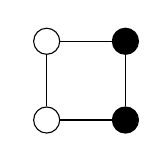
\begin{tikzpicture}
        \node[shape=circle,draw=black,fill=black] (A) at (1,0){};
        \node[shape=circle,draw=black,fill=black] (B) at (1,1){};
        \node[shape=circle,draw=black] (C) at (0,1){}; 
        \node[shape=circle,draw=black] (D) at (0,0){};
        \path [-](A) edge node[left]{} (B);
        \path [-](B) edge node[left]{} (C);
        \path [-](C) edge node[left]{} (D);
        \path [-](D) edge node[left]{} (A);
    \end{tikzpicture}
    \qquad
    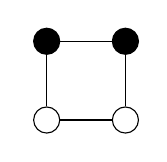
\begin{tikzpicture}
        \node[shape=circle,draw=black] (A) at (1,0) {};
        \node[shape=circle,draw=black,fill=black] (B) at (1,1) {};
        \node[shape=circle,draw=black,fill=black] (C) at (0,1) {};
        \node[shape=circle,draw=black] (D) at (0,0) {};
        \path [-](A) edge node[left]{} (B);
        \path [-](B) edge node[left]{} (C);
        \path [-](C) edge node[left]{} (D);
        \path [-](D) edge node[left]{} (A);
    \end{tikzpicture}
    \qquad
    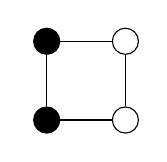
\begin{tikzpicture}
        \node[shape=circle,draw=black] (A) at (1,0) {};
        \node[shape=circle,draw=black] (B) at (1,1) {};
        \node[shape=circle,draw=black,fill=black] (C) at (0,1) {};
        \node[shape=circle,draw=black,fill=black] (D) at (0,0) {};
        \path [-](A) edge node[left]{} (B);
        \path [-](B) edge node[left]{} (C);
        \path [-](C) edge node[left]{} (D);
        \path [-](D) edge node[left]{} (A);
    \end{tikzpicture}
    \qquad
    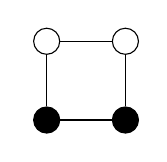
\begin{tikzpicture}
        \node[shape=circle,draw=black,fill=black] (A) at (1,0) {};
        \node[shape=circle,draw=black] (B) at (1,1) {};
        \node[shape=circle,draw=black] (C) at (0,1) {};
        \node[shape=circle,draw=black,fill=black] (D) at (0,0) {};
        \path [-](A) edge node[left]{} (B);
        \path [-](B) edge node[left]{} (C);
        \path [-](C) edge node[left]{} (D);
        \path [-](D) edge node[left]{} (A);
    \end{tikzpicture}
\end{equation}
will be considered equivalent. Let $G=\langle g\rangle$ the cyclic 
group of order four. Let $X$ be 
the set of colorings of the square. Then 
$|X|=16$. 

Let $g$ act on $X$ by anti-clockwise rotations  
of 90\textdegree. All the colorings of~\eqref{eq:orbita} belong to the same orbit. 
Another orbit of $X$ is
\[
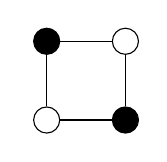
\begin{tikzpicture}
    \node[shape=circle,draw=black,fill=black] (A) at (1,0) {};
    \node[shape=circle,draw=black] (B) at (1,1) {};
    \node[shape=circle,draw=black,fill=black] (C) at (0,1) {};
    \node[shape=circle,draw=black] (D) at (0,0) {};
    \path [-](A) edge node[left]{} (B);
    \path [-](B) edge node[left]{} (C);
    \path [-](C) edge node[left]{} (D);
    \path [-](D) edge node[left]{} (A);
\end{tikzpicture}
\qquad
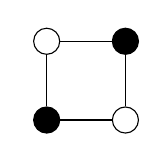
\begin{tikzpicture}
    \node[shape=circle,draw=black] (A) at (1,0) {};
    \node[shape=circle,draw=black,fill=black] (B) at (1,1) {};
    \node[shape=circle,draw=black] (C) at (0,1) {};
    \node[shape=circle,draw=black,fill=black] (D) at (0,0) {};
    \path [-](A) edge node[left]{} (B);
    \path [-](B) edge node[left]{} (C);
    \path [-](C) edge node[left]{} (D);
    \path [-](D) edge node[left]{} (A);
\end{tikzpicture}
\]

Cauchy--Frobenius--Burnside theorem states that
there are  
\[
\frac{1}{|G|}\sum_{x\in G}|\Fix(x)|
\]
orbits. 

For each $x\in G=\{1,g,g^2,g^3\}$ we compute $\Fix(x)$. The identity fixes 
the 16 elements of $X$, both 
$g$ and  $g^3$ fix only two elements of $X$ and 
$g^2$ fixes four elements of $X$. For example, 
the elements of $X$ fixed by $g^2$ are 
\[
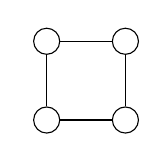
\begin{tikzpicture}
    \node[shape=circle,draw=black] (A) at (1,0){};
    \node[shape=circle,draw=black] (B) at (1,1){};
    \node[shape=circle,draw=black] (C) at (0,1){}; 
    \node[shape=circle,draw=black] (D) at (0,0){};
    \path [-](A) edge node[left]{} (B);
    \path [-](B) edge node[left]{} (C);
    \path [-](C) edge node[left]{} (D);
    \path [-](D) edge node[left]{} (A);
\end{tikzpicture}
\qquad
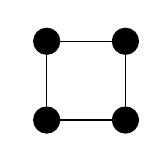
\begin{tikzpicture}
    \node[shape=circle,draw=black,fill=black] (A) at (1,0) {};
    \node[shape=circle,draw=black,fill=black] (B) at (1,1) {};
    \node[shape=circle,draw=black,fill=black] (C) at (0,1) {};
    \node[shape=circle,draw=black,fill=black] (D) at (0,0) {};
    \path [-](A) edge node[left]{} (B);
    \path [-](B) edge node[left]{} (C);
    \path [-](C) edge node[left]{} (D);
    \path [-](D) edge node[left]{} (A);
\end{tikzpicture}
\qquad
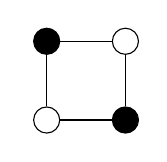
\begin{tikzpicture}
    \node[shape=circle,draw=black,fill=black] (A) at (1,0) {};
    \node[shape=circle,draw=black] (B) at (1,1) {};
    \node[shape=circle,draw=black,fill=black] (C) at (0,1) {};
    \node[shape=circle,draw=black] (D) at (0,0) {};
    \path [-](A) edge node[left]{} (B);
    \path [-](B) edge node[left]{} (C);
    \path [-](C) edge node[left]{} (D);
    \path [-](D) edge node[left]{} (A);
\end{tikzpicture}
\qquad
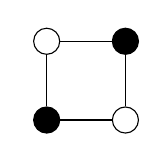
\begin{tikzpicture}
    \node[shape=circle,draw=black] (A) at (1,0) {};
    \node[shape=circle,draw=black,fill=black] (B) at (1,1) {};
    \node[shape=circle,draw=black] (C) at (0,1) {};
    \node[shape=circle,draw=black,fill=black] (D) at (0,0) {};
    \path [-](A) edge node[left]{} (B);
    \path [-](B) edge node[left]{} (C);
    \path [-](C) edge node[left]{} (D);
    \path [-](D) edge node[left]{} (A);
\end{tikzpicture}
\]
Thus $X$ is the union of  
\[
\frac{1}{|G|}\sum_{x\in G}|\Fix(x)|=\frac{1}{4}(16+2+4+2)=6
\]
orbits. 
\end{example}

\begin{exercise}
    In how many ways (up to symmetry) can you
    arrange eight non-attacking rooks on a chessboard? Symmetries 
    are given by the dihedral group $\D_4$ of eight elements.
\end{exercise}

There are 5282 ways (up to symmetry) to arrange 
eight non-attacking rooks on a chessboard. 

\topic{Commuting probability}

\index{Group commutativity}
For a finite group $G$, let $\cp(G)$ be the probability 
that two random elements of $G$ commute. This number
is also known as the \textbf{commutativity} of $G$. 
As an application of Cauchy--Frobenius--Burnside theorem, we
prove that 
$\cp(G)=k/|G|$, where $k$ is the number of conjugacy classes
of $G$. Let 
\[
C=\{(x,y)\in G\times G:xy=yx\}.
\]
We claim that  
    \[
    \cp(G)=\frac{|C|}{|G|^2}=\frac{k}{|G|}.
    \]

Let $G$ act on $G$ by conjugation. 
    By Cauchy--Frobenius--Burnside theorem, 
    \[
    k=\frac{1}{|G|}\sum_{g\in G}|\Fix(g)|=\frac{1}{|G|}\sum_{g\in G}|C_G(g)|=\frac{|C|}{|G|},
    \]
    as $\Fix(g)=\{x\in G:gxg^{-1}=x\}=C_G(g)$ and $\sum_{g\in G}|C_G(g)|=|C|$. 
Alternatively, using Theorem \ref{thm:Frobenius_tau(g)} for $g = 1$ we get
\[
    \cp(G) = \frac{\tau(1)}{|G|^2} = \frac{1}{|G|}\sum_{\chi \in \Irr(G)} 1 = \frac{|C|}{|G|}.
\]
\begin{theorem}
\index{Theorem!5/8}
\label{thm:5/8}
    If $G$ is a non-abelian finite group, then $\cp(G)\leq5/8$.
\end{theorem}

\begin{proof}
%
%    We now claim that $k/|G|\leq 5/8$ if $G$ is non-abelian.
    Let $y_1,\dots,y_m$ the representatives of conjugacy classes of $G$ 
    of size $\geq2$. By the class equation, 
    \[
    |G|=|Z(G)|+\sum_{i=1}^m(G:C_G(y_i))\geq |Z(G)|+2m.
    \]
    Thus $m\leq(1/2)(|G|-|Z(G)|)$ and hence 
    \[
    k=|Z(G)|+m\leq |Z(G)|+\frac12(|G|-|Z(G)|)=\frac12(|Z(G)|+|G|).
    \]
    Since $G$ is non-abelian, $G/Z(G)$ is not cyclic. In particular, 
    $(G:Z(G))\geq4$. Therefore
    \[
    k\leq\frac12(|Z(G)|+|G|)\leq\frac12\left(\frac14+1\right)|G|,
    \]
    that is $k/|G|\leq 5/8$. 
\end{proof}

\begin{exercise}\
\begin{enumerate}
    \item Prove that $\cp(Q_8)=5/8$. 
    \item Prove that $\cp(\Alt_5)=1/12$. 
\end{enumerate}
\end{exercise}

\begin{exercise}
    Let $G$ be a finite non-abelian group and $p$ be the smallest prime number
    dividing $|G|$. Prove that $\cp(G)\leq (p^2+p-1)/p^3$. Moreover, 
    the equality holds if and only if $(G:Z(G))=p^2$. 
\end{exercise}

\begin{exercise}
    Let $G$ be a finite group and $H$ be a subgroup of $G$.
    \begin{enumerate}
        \item $\cp(G)\leq\cp(H)$.
        \item If $H$ is normal in $G$, then $\cp(G)\leq\cp(G/H)\cp(H)$.
    \end{enumerate}
\end{exercise}

Degrees of irreducible characters give a lower bound:

\begin{proposition}
If $G$ is a finite group, then
\[
\cp(G)\geq\left(\frac{\sum_{\chi\in\Irr(G)}\chi(1)}{|G|}\right)^2.
\]
\end{proposition}

\begin{proof}
    Let $k$ be the number of conjugacy classes of $G$.
    By Cauchy--Schwarz inequality, 
    \begin{align*}
        \left(\sum_{\chi\in\Irr(G)}\chi(1)\right)^2
        &\leq\left(\sum_{\chi\in\Irr(G)}\chi(1)^2\right)\left(\sum_{\chi\in\Irr(G)}1\right)
        =\left(\sum_{\chi\in\Irr(G)}\chi(1)^2\right)k=|G|k.
    \end{align*}
    From this, the claim follows.
\end{proof}

Using basic facts about irreducible characters, 
we obtain a generalization of Theorem \ref{thm:5/8}. 

\begin{theorem}
\label{thm:[GG]}
    Let $G$ be a finite group. Then
    \[
    |[G,G]|\leq 3/(4\cp(G)-1).
    \]
\end{theorem}

\begin{proof}
    For $n\in\Z_{>0}$, let $\rho_n$ be the number
    of irreducible characters of degree $n$. Then 
    the number of conjugacy classes of $G$ is $k=\sum_{i\geq1}\rho_i$
    and $|G|=\sum_{i\geq1}i^2\rho_i$. 
    It follows that 
    \begin{align*}
    |G|-\rho_1 &=\sum_{i\geq 2}i^2\rho_i\geq 4\sum_{i\geq2}\rho_i
    =4(k-\rho_1)=4(|G|\cp(G)-\rho_1).
    \end{align*}
    Since $\rho_1=(G:[G,G])$, 
    \[
    \cp(G)\leq \frac14+\frac34\frac{\rho_1}{|G|}=\frac14+\frac3{4|[G,G]|}.
    \]
    From this, the claim follows. 
\end{proof}

\begin{exercise}
    \label{xca:5/8}
    Use Theorem \ref{thm:[GG]} to prove Theorem \ref{thm:5/8}.
\end{exercise}

Theorem \ref{thm:[GG]} 
can also be used to
prove similar statements. 

\begin{exercise}
    \label{xca:cp_NS}
    Let $G$ be a finite group. Prove the following statements:
    \begin{enumerate}
        \item If $\cp(G)>1/2$, then $G$ is nilpotent.
        \item If $\cp(G)>21/80$, then $G$ is solvable. 
    \end{enumerate}
\end{exercise}

In the following exercise, we will discuss the notion 
of isoclinic groups. We first need
a preliminary result:

\begin{exercise}
\index{Commutator map}
\label{xca:commutator_map}
    Let $G$ be a group. Prove that the commutator map
    \[
    c_G\colon G/Z(G)\times G/Z(G)\to [G,G],
    \quad
    c_G(xZ(G),yZ(G))=[x,y],
    \]
    is well-defined. 
\end{exercise}

The idea is that two groups are said to be isoclinic 
if their commutator functions are somewhat equal. 

\begin{exercise}
\index{Isoclinism}
\label{xca:isoclinism}
    Let $G$ and $H$ be groups. 
    A pair $(\sigma,\tau)$ of maps is an \textbf{isoclinism}
    between $G$ and $H$ if 
    $\sigma\colon G/Z(G)\to H/Z(H)$ and  
    $\tau\colon [G,G]\to [H,H]$ are group isomorphisms and 
    the diagram
    \begin{equation}
    \label{eq:isoclinism}
    \begin{tikzcd}
	{G/Z(G)\times G/Z(G)} & {H/Z(H)\times H/Z(H)} \\
	{[G,G]} & {[H,H]}
	\arrow["{\sigma\times\sigma }", from=1-1, to=1-2]
	\arrow["{c_H}", from=1-2, to=2-2]
	\arrow["{c_G}"', from=1-1, to=2-1]
	\arrow["\tau"', from=2-1, to=2-2]
    \end{tikzcd}
    \end{equation} 
    commutes. We write $G\sim H$ when there exists 
    an isoclinism between $G$ and $H$. 
    
    Prove the following statements:
    \begin{enumerate}
        \item If $G\simeq H$, then $G\sim H$.
        \item If $G\sim H$, then $\cp(G)=\cp(H)$. 
    \end{enumerate}
\end{exercise}

\begin{exercise}
\label{xca:isoclinism_simple}
    Let $S$ be a non-abelian simple group and
    $G$ be a group such that $G\sim S$. Prove that 
    $G\simeq S\times A$ for some abelian group $A$.
\end{exercise}

\begin{exercise}
\label{xca:isoclinism_factorization}
    Let $H$ be a subgroup of $G$. If $G=HZ(G)$, then $G\sim H$. 
    Conversely, if $G\sim H$ and $H$ is finite, then 
    $G=HZ(G)$. 
\end{exercise}

The following theorem appeared in 1970 as a problem in 
volume 13 of the \emph{Canadian Math. Bulletin}. The solution
appeared in 1973. 
Iv\'an Sadosfchi Costa found the proof we present here. 

\begin{theorem}[Dixon]
    \index{Dixon's theorem}
    The commuting probability of every finite 
    non-abelian simple group is at most $1/12$. 
   %If $G$ is a finite non-abelian simple group, then $\cp(G)\leq1/12$.
\end{theorem}

\begin{proof}
Let $G$ be a finite non-abelian simple group. We claim that 
$\cp(G)\leq1/12$. 

We first assume that $\cp(G)>1/12$. Since
$G$ is a non-abelian simple group, 
the identity of $G$ is the only central element of $G$. 
Let us assume first that there is a conjugacy class of $G$ of size $m$, where
$m$ is such that $1<m\leq 12$. Then $G$ is a transitive subgroup of $\Sym_m$.
For these groups, the problem is easy: we show that there are no non-abelian simple groups
that act transitively on sets of size $m\in\{2,\dots,12\}$ with commuting
probability $>1/12$. To do this, we list these transitive groups and their commuting
probabilities and verify that all commuting probabilities are $\leq
1/12$:
\begin{lstlisting}
gap> l := AllTransitiveGroups(NrMovedPoints, [2..12], \\
> IsAbelian, false, IsSimple, true);;
[ A5, L(6) = PSL(2,5) = A_5(6), A6, 
  L(7) = L(3,2), A7, L(8)=PSL(2,7), A8, 
  L(9)=PSL(2,8), A9, A_5(10), L(10)=PSL(2,9), 
  A10, L(11)=PSL(2,11)(11), M(11), A11, A_5(12), 
  L(2,11), M_11(12), M(12), A12 ]
gap> List(l, CommutingProbability);           
[ 1/12, 1/12, 7/360, 1/28, 1/280, 1/28, 1/1440, 
  1/56, 1/10080, 1/12, 7/360, 1/75600, 2/165, 
  1/792, 31/19958400, 1/12, 2/165, 1/792, 1/6336, 
  43/239500800 ]
gap> ForAny(l, x->CommutingProbability(x)>1/12);
false
\end{lstlisting}

Now assume that all non-trivial conjugacy classes of $G$ have at least 13 elements. 
Then the class equation implies that
\begin{align*}
	|G|&\geq \frac{13}{12}|G|-12,
\end{align*}
and therefore $|G|\leq 144$. Thus one needs to check what happens with groups
of order $\leq 144$. 
But we know that the only non-abelian simple group of size
$\leq 144$ is the alternating simple group $\Alt_5$.
\begin{lstlisting}
gap> AllGroups(Size, [2..144], \\
> IsAbelian, false, \\
> IsSimple, true);
[ Alt( [ 1 .. 5 ] ) ]
\end{lstlisting}    
This completes the proof. 
\end{proof}

The alternating group $\Alt_5$ is important in this setting:

\begin{theorem}[Guralnick--Robinson]
    \index{Guralnick--Robinson theorem}
    If $G$ is a finite non-solvable group such that $\cp(G)>3/40$, then
    $G\simeq\Alt_5\times T$ for some abelian group 
    $T$ and $\cp(G)=1/12$. 
\end{theorem}

The proof appears in~\cite{MR2228209}.

Results on probability of commuting elements generalize in other directions. 
In~\cite{MR230809,MR276325,MR313378,MR369512}, 
Thompson proved the following result:

\begin{theorem}[Thompson]
\index{Thompson's theorem}
    If $G$ is a finite group such that 
    every pair of elements of $G$ generate
    a solvable group, then $G$ is solvable. 
\end{theorem}

The proof uses the classification of finite simple groups (CFSG). A simpler
proof independent of the CFSG appears in~\cite{MR1346207}.

There is a probabilistic version of Thompson's theorem:

\begin{theorem}[Guralnick--Wilson]
    \index{Guralnick--Wilson theorem}
    Let $G$ be a finite group.
    \begin{enumerate}
        \item If the probability that two random elements of $G$ 
        generate a solvable group is $>11/30$, then $G$ is solvable. 
        \item If the probability that two random elements of $G$ 
        generate a nilpotent group is $>1/2$, then $G$ is nilpotent.
        \item If the probability that two random elements of $G$ 
        generate a group of odd order is $>11/30$, then $G$ has odd order.
    \end{enumerate}
\end{theorem}

The proof uses the CFSG and appears in~\cite{MR1770615}.

\topic{Jordan's theorem and applications}

We now follow~\cite{MR1997347} to present other applications. 

\begin{theorem}[Jordan]
\index{Jordan's theorem}
    Let $G$ be a non-trivial finite group. If $G$ acts transitively 
    on a finite set $X$ and $|X|>1$, then there exists 
    $g\in G$ with no fixed points.
\end{theorem}

\begin{proof}
    Cauchy--Frobenius--Burnside theorem implies that
    \[
    1=\frac{1}{|G|}\sum_{g\in G}|\Fix(g)|=\frac{1}{|G|}\left(|X|+\sum_{g\ne 1}|\Fix(g)|\right).
    \]
    If every $g\in G\setminus\{1\}$ contains at least one fixed-point, then
    \[
    1=\frac{1}{|G|}\left(|X|+\sum_{g\ne 1}|\Fix(g)|\right)\geq \frac{1}{|G|}(|X|+|G|-1)=1+\frac{|X|-1}{|G|}
    \]
    and thus $|X|\leq1$, a contradiction. 
\end{proof}

\begin{corollary}
    Let $G$ be a finite group and $H$ be a proper subgroup of $G$. 
    Then $G\ne\cup_{g\in G}gHg^{-1}$.
\end{corollary}

\begin{proof}
    The group $G$ acts transitively by left multiplication on $X=G/H$. The stabilizer
    of $xH$ is 
    \[
    G_{xH}=\{g\in G:gxH=xH\}=xHx^{-1}.
    \]
    Since $H\ne G$, it follows that $|X|=|G/H|>1$. Jordan's theorem now implies
    that there exists $g\in G$ with no fixed-points, that is 
    there is an element $g\in G$ such that $g\not\in\cup_{x\in G}xHx^{-1}$. 
\end{proof}

Let $G$ be a finite group. We say that the conjugacy classes $C$ and $D$ 
\textbf{commute} if there exist 
$c\in C$ and $d\in D$ such that $[c,d]=1$. 
Note that $C$ and $D$ commute if and only if for all $c\in C$ there exists $d\in D$ 
such that $[c,d]=1$. 

\begin{corollary}[Wildon]
\index{Wildon's theorem}
    Let $G$ be a finite group and $C$ be a conjugacy class of $G$. 
    Then $|C|=1$ if and only if $C$ commutes 
    with every conjugacy class of $G$.
\end{corollary}
    
\begin{proof}
    We prove $\impliedby$. 
    Assume that $C$ commutes with every conjugacy class of $G$. 
    Let $c\in C$ and $H=C_G(c)$. Then $H\cap D\ne\emptyset$ for every conjugacy class
    $D$. We claim that $G=\cup_{g\in G}gHg^{-1}$. In fact, let $x\in G$. Then
    $x\in D$ 
    for some conjugacy class $D$. 
    Let 
    $h\in H\cap D$. There exists $y\in G$ such that $h=yxy^{-1}$, that is
    $x=y^{-1}hy\in \cup_{g\in G}gHg^{-1}$. By Jordan's theorem,  
    $H=G$. Thus $c$ is central and hence $C=\{c\}$. 
    
    We now prove $\implies$. If $C=\{c\}$, then $c\in Z(G)$ and $C$ commute with every 
    conjugacy class of~$G$. 
\end{proof}

With the CFSG one proves a result similar to that of Jordan. 

\begin{theorem}[Fein--Kantor--Schacher]
    \index{Fein--Kantor--Schacher theorem}
    Let $G$ be a non-trivial finite group. If $G$ acts transitively
    on a finite set $X$ and $|X|>1$, then
    there exist a prime number $p$ and an element $g\in G$ with no fixed-points
    with order a power of $p$.
\end{theorem}

The proof appears in~\cite{MR636194}. 

\topic{Derangements: Cameron--Cohen theorem}

\index{Derangements}
Let $G$ be a finite group that acts faithfully and transitively 
on a finite set $X$, say 
$G\leq\Sym_n$, where $X=\{1,2,\dots,n\}$. Let 
$G_0$ be the set of elements $g\in G$ with no fixed-points, 
that is $g(x)\ne x$ for all $x\in X$. 
Such permutations are known as \textbf{derangements}. 
Let $c_0=|G_0|/|G|$. 

\begin{theorem}[Cameron--Cohen]
    \index{Cameron--Cohen theorem}
    If $G$ is a subgroup of $\Sym_n$ that acts transitively on 
    $\{1,\dots,n\}$, then $c_0\geq\frac{1}{n}$.
\end{theorem}

\begin{proof}
    Let $X=\{1,\dots,n\}$. By definition, the rank of $G$ is the number
    of orbitals of $G$ on $X$. It follows that the rank is $\geq2$, as
    $X\times X$ decomposes as 
    \[
    X\times X=\Delta\cup\left((X\times X)\setminus\Delta\right)
    \]
    Let $\chi(g)=|\Fix(g)|$ and $G_0=\{g\in G:\chi(g)=0\}$. If $g\not\in G_0$, then $1\leq\chi(g)\leq n$. Since  
    $(\chi(g)-1)(\chi(g)-n)\leq 0$,
    \[
    \frac{1}{|G|}\sum_{g\in G\setminus G_0}(\chi(g)-1)(\chi(g)-n)\leq 0.
    \]
    On the one hand, 
    \begin{align*}
    \frac{1}{|G|}\sum_{g\in G}(\chi(g)&-1)(\chi(g)-n)\\
    &=\frac{1}{|G|}\left\{\sum_{g\in G_0}+\sum_{g\in G\setminus G_0}\right\}(\chi(g)-1)(\chi(g)-n)\\
    &\leq n\frac{|G_0|}{|G|}=nc_0.
    \end{align*}
    On the other hand, since the rank of $G$ is $\geq2$, 
    \begin{equation}
        \label{eq:CameronCohen}
        2-\frac{n+1}{|G|}\sum_{g\in G}\chi(g)+n\leq 
        \frac{1}{|G|}\sum_{g\in G}(\chi(g)-1)(\chi(g)-n)\leq nc_0.
    \end{equation}
    Since $G$ is transitive on $X$, Cauchy--Frobenius--Burnside theorem implies that
    $\sum_{g\in G}\chi(g)=|G|$. Thus $2-(n+1)+n\leq nc_0$ and hence
    $1/n\leq c_0$. 
\end{proof}

Cameron--Cohen theorem contains another claim: If
$n$ is not the power of a prime number, then 
$c_0>1/n$. The proof uses Frobenius' theorem. 

With the CFSG the bound in 
Cameron--Cohen theorem can be improved:

\begin{theorem}[Guralnick--Wan]
    \index{Guralnick--Wan theorem}
    Let $G$ be a finite transitive group of degree $n\geq2$. If $n$ 
    is not a power of a prime number and 
    $G\ne\Sym_n$ for $n\in\{2,4,5\}$, then $c_0\geq 2/n$.
\end{theorem}

The proof appears in~\cite{MR1484879} and uses
the classification of finite 2-transitive groups, 
which depends on the CFSG. 



